\documentclass[11pt,a4paper,openany]{book}
\usepackage[margin=24mm]{geometry}
\usepackage{fontspec}
\IfFontExistsTF{Noto Serif}{\setmainfont{Noto Serif}}{\setmainfont{DejaVu Serif}}
\usepackage{amsmath,amssymb,tikz,enumitem,microtype}
\usepackage[hidelinks]{hyperref}
\setlength{\parindent}{0pt}
\setlength{\parskip}{6pt}
\setlist[enumerate]{leftmargin=*,itemsep=8pt}
\setlength{\emergencystretch}{2em}

\renewcommand{\contentsname}{Contents}
\begin{document}
\title{V-TALENT 2045\\ PHY101-B --- Geometry, trigonometry and graphs\\\large Level 1 \textbar{} Mathematics for Physics}
\author{Dr. Dang Minh Tuan -- TS. Đặng Minh Tuấn}
\date{2026 \textbar{} Draft v1.0}
\maketitle
\tableofcontents
\chapter*{How to study}
Grades 8–9. Prerequisites: PHY101-A, basic geometry and algebra. Work in degrees unless otherwise stated; no calculus is required.

Predict first; draw a model; reproduce worked examples without looking; solve independently and check the solutions at the back. Original teaching content; source links are further reading, not copied text. Draft pending independent review.
\chapter{Similarity and optical geometry}
\section{Learning objectives}
Use similar triangles to infer inaccessible distances and distinguish a ray model from a real image.
\section{Theory and derivations}
Triangles with equal corresponding angles are similar; ratios of corresponding sides are equal. Draw the geometry before forming ratios, label corresponding sides and use consistent length units. For a vertical object of height H on level ground with shadow length S, a reference rod of height h and shadow s at the same instant gives $H/S=h/s$ when the light rays are effectively parallel. A nearby lamp generally violates this parallel-ray model.

For a pinhole camera, straight rays through a tiny aperture connect the top of the object to the bottom of the screen. Similar triangles give $|h_i|/h_o=d_i/d_o$, where distances are positive magnitudes measured from the pinhole. In the signed-height convention, $h_i/h_o=-d_i/d_o$. This is geometric projection, not the thin-lens equation. A finite aperture produces blur; diffraction also limits the resolution of very small apertures.

Reflection at a plane mirror follows equal angles measured from the normal, not the mirror surface. A virtual image lies as far behind the mirror as the object is in front. Construct the apparent straight path to that image; its intersection with the mirror gives the reflection point. This construction assumes a flat mirror and unobstructed rays.
\begin{center}
\begin{tikzpicture}[scale=.85]\draw[dashed](-4,0)--(3,0);\draw[->,thick](-3,0)--(-3,2)node[above]{$h_o$};\draw[thick](0,-2)--(0,-.08)(0,.08)--(0,2);\draw[thick](2,-2)--(2,2);\draw[blue](-3,2)--(2,-1.333);\draw[->,thick](2,0)--(2,-1.333)node[below]{$h_i$};\node at(-1.5,-.3){$d_o$};\node at(1,.3){$d_i$};\end{tikzpicture}
\end{center}
\section{Worked examples}
\subsection*{Example 1.1}
A 1.2 m rod casts a 0.8 m shadow; a tree casts a 7.6 m shadow at the same instant. Find height.

\textbf{Solution.} $H/7.6=1.2/0.8$, hence $H=11.4$ m. The result assumes level ground and parallel rays.
\subsection*{Example 1.2}
A 1.8 m object stands 6 m from a pinhole. The screen is 40 mm behind it. Find image height.

\textbf{Solution.} $d_i=0.040$ m. $h_i=-1.8(0.040)/6=-0.012$ m, or 12 mm inverted.
\section{Investigation}
Make a paper pinhole viewer for a brightly lit indoor object (never look at the Sun). Measure image height at two screen distances, predict the ratio, and discuss blur.
\section{Modern application and transfer}
A simplified calibrated camera has effective projection distance 5 mm. A 0.6 m marker produces an image 1.5 mm high, implying distance 2 m. This supports machine-vision distance estimation when object size is known and orientation is appropriate. Real cameras require lens calibration and distortion correction.
\section{Source-guided reading}
SJ ch. 29 (geometric optics), p. 106; source catalogue SJ-29; optical reading is an extension.
\section{Independent practice}
\begin{enumerate}
\item \textbf{PHY101-B-1.1}. A 1.5 m pole casts a 2 m shadow; a tower casts 18 m. Find tower height under the same conditions.
\item \textbf{PHY101-B-1.2}. A pinhole image of a 30 cm object at distance 2 m is 6 mm high. Find screen distance.
\item \textbf{PHY101-B-1.3}. A ray makes 25 degrees with a plane mirror surface. Find incidence and reflection angles.
\item \textbf{PHY101-B-1.4}. A lamp is at height 3 m, a 1 m rod stands 2 m horizontally from the lamp base. On level ground find the rod's shadow length beyond its foot.
\end{enumerate}
\chapter{Trigonometry, vectors and navigation}
\section{Learning objectives}
Resolve a vector into perpendicular components; reconstruct magnitude and direction; use triangle inequalities.
\section{Theory and derivations}
For a right triangle with hypotenuse c and angle $\theta$, $\sin\theta=\text{opposite}/c$, $\cos\theta=\text{adjacent}/c$, $\tan\theta=\text{opposite}/\text{adjacent}$. Pythagoras yields $\sin^2\theta+\cos^2\theta=1$. A vector of magnitude A at angle $\theta$ counterclockwise from positive x has components $A_x=A\cos\theta$, $A_y=A\sin\theta$. A component may be negative; the magnitude cannot.

To add vectors use head-to-tail construction or add matching components. Resultant magnitude is $\sqrt{R_x^2+R_y^2}$. For two vectors of lengths a and b, $|a-b|\le R\le a+b$, with equality for collinear vectors. The tangent ratio alone does not identify a quadrant. For example, a vector with both components negative lies in quadrant III even when its tangent ratio is positive. Bearings are often measured clockwise from north, unlike mathematical angles.

In a uniform current, ground velocity is the vector sum of the vessel's velocity relative to water and the current. If a crossing must be perpendicular to the shore, the upstream component must cancel the current. A direct crossing is impossible if current speed is at least the vessel's speed (at equality no across-river component remains). A shortest-time crossing instead maximises the perpendicular component and may drift.
\begin{center}
\begin{tikzpicture}[scale=.8]\draw[->](0,0)--(5,0)node[right]{$x$};\draw[->](0,0)--(0,4)node[above]{$y$};\draw[->,very thick,blue](0,0)--(4,3)node[above]{$\vec A$};\draw[dashed](4,3)--(4,0);\node at(2,-.3){$A_x$};\node[right]at(4,1.5){$A_y$};\draw(1,0)arc(0:36.87:1);\end{tikzpicture}
\end{center}
\section{Worked examples}
\subsection*{Example 2.1}
A 10 N force points 30 degrees above horizontal. Find components.

\textbf{Solution.} $F_x=10\cos30^\circ=5\sqrt3\approx8.66$ N; $F_y=10\sin30^\circ=5$ N.
\subsection*{Example 2.2}
A drone flies 3 km east then 4 km north. Find net displacement magnitude and direction.

\textbf{Solution.} $R=\sqrt{3^2+4^2}=5$ km; angle north of east $\arctan(4/3)\approx53.13^\circ$. Total path length is 7 km.
\section{Investigation}
Use graph paper to add two displacement arrows at different angles. Measure resultant length and compare with component calculation. Discuss scale-reading error.
\section{Modern application and transfer}
A mobile robot's wheel odometry estimates 1.2 m east and 0.5 m north. Its straight displacement is 1.3 m. If wheels slip, component estimates become biased; an independent visual landmark can correct the estimate.
\section{Source-guided reading}
SJ §§5.1–5.2, pp. 20–23 (vector concepts; defer calculus and cross product).
\section{Independent practice}
\begin{enumerate}
\item \textbf{PHY101-B-2.1}. Resolve a 20 N force at 60 degrees above +x.
\item \textbf{PHY101-B-2.2}. Add vectors (-3,4) and (5,-1) in metres; find magnitude.
\item \textbf{PHY101-B-2.3}. A boat moves at 5 m/s relative to water; current is 3 m/s. Find across speed when heading to land opposite.
\item \textbf{PHY101-B-2.4}. Two forces have magnitudes 6 N and 8 N. Can their resultant be 1 N? Can it be 10 N? Explain.
\end{enumerate}
\chapter{Graphs, gradients and accumulated quantities}
\section{Learning objectives}
Read axes and units, distinguish slope from height and find signed areas using geometry.
\section{Theory and derivations}
A graph is a representation of ordered pairs, not a drawing of the physical path. Label each axis with quantity and unit. For a straight segment the slope is $\Delta y/\Delta x$ and depends on the axes. On an x–t graph slope gives velocity; on a v–t graph slope gives acceleration. Intercept describes an initial or offset value, not necessarily an error. Visual steepness depends on plotting scale, so calculate slope numerically.

For a constant velocity, displacement is rectangle area $v\Delta t$. For a velocity varying linearly, the signed trapezium area is $(v_1+v_2)\Delta t/2$. If the velocity crosses zero, split the interval there: signed areas give displacement, absolute areas give distance. Likewise, power–time area gives energy for piecewise constant or linear power. Check the product of axis units to interpret area.

A linear model $y=ax+b$ should be tested on multiple measurements. Draw a trend line without forcing it through the origin unless the physics requires that and the data support it. Use two separated points on the fitted line for slope; do not connect noisy observations as if each fluctuation were a physical law. A graph may support a model over its measured range without establishing validity outside it.
\begin{center}
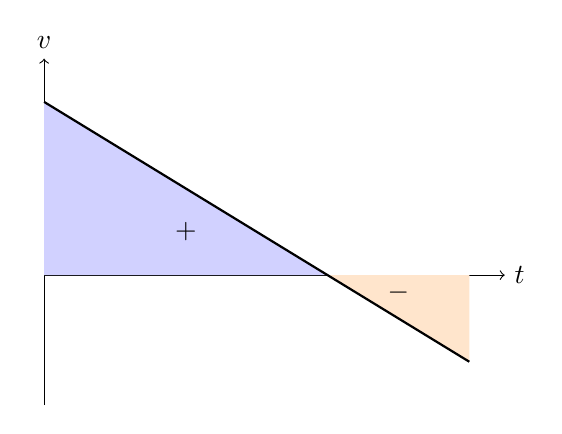
\begin{tikzpicture}[x=.9cm,y=.55cm]\draw[->](0,0)--(6.5,0)node[right]{$t$};\draw[->](0,-3)--(0,5)node[above]{$v$};\fill[blue!18](0,0)--(0,4)--(4,0)--cycle;\fill[orange!20](4,0)--(6,-2)--(6,0)--cycle;\draw[thick](0,4)--(6,-2);\node at(2,1){$+$};\node at(5,-.4){$-$};\end{tikzpicture}
\end{center}
\section{Worked examples}
\subsection*{Example 3.1}
Velocity decreases uniformly from 4 to -2 m/s in 6 s. Find acceleration, displacement and distance.

\textbf{Solution.} $a=(-2-4)/6=-1$ m/s$^2$. Zero at 4 s. Positive area 8 m, negative area -2 m: displacement 6 m, distance 10 m.
\subsection*{Example 3.2}
A device uses 20 W for 10 s then power increases linearly from 20 to 60 W over 5 s. Find energy.

\textbf{Solution.} $E=20(10)+(20+60)5/2=400$ J.
\section{Investigation}
Use a phone video of a toy car, record positions at equal intervals, plot x versus t and estimate slopes. Compare intervals rather than assuming constant speed.
\section{Modern application and transfer}
A battery logger records power versus time. Summing trapezium areas estimates energy usage, useful for planning portable instruments. Sparse sampling can miss rapid spikes; compare sampling intervals before relying on an energy budget.
\section{Source-guided reading}
SJ §§4.2–4.3, pp. 15–16; SW graph reading locator from catalogue (not rechecked).
\section{Independent practice}
\begin{enumerate}
\item \textbf{PHY101-B-3.1}. Position rises from 2 m to 14 m over 3 s on a straight x–t segment. Find velocity.
\item \textbf{PHY101-B-3.2}. Velocity is 3 m/s for 4 s then -2 m/s for 3 s. Find displacement and distance.
\item \textbf{PHY101-B-3.3}. A U–I graph is linear through (0.1 A,2 V) and (0.3 A,6 V). Find slope and intercept.
\item \textbf{PHY101-B-3.4}. A 100 W lamp runs for 15 min. Express energy in J and Wh.
\end{enumerate}
\chapter{Geometric optimization and model transfer}
\section{Learning objectives}
Optimize simple distances and areas using geometry; distinguish a mathematical optimum from a constrained physical optimum.
\section{Theory and derivations}
The triangle inequality says a straight line is the shortest distance between two points in an unobstructed Euclidean plane. For a route from A to B touching a straight mirror line, reflect B across the line to B'. For every point P on the line, $AP+PB=AP+PB'\ge AB'$. Equality holds when P lies on segment AB'. Check whether the allowed mirror segment contains P. The result minimizes travel time only if speed is constant on both legs.

For a rectangle of fixed perimeter 2S, area $A=x(S-x)=S^2/4-(x-S/2)^2$ is maximal at $x=S/2$. The square wins because the subtracted square is nonnegative. If a required minimum width, material constraint or different edge costs are present, the feasible interval or objective changes. Do not apply an unconstrained optimum blindly.

For a fixed force magnitude F and displacement s, work $W=Fs\cos\theta$ is maximal when the force points along displacement. But if the applied force changes normal reaction, friction also changes: maximal applied work need not imply maximal net acceleration. This distinction motivates constrained dynamics in PHY202-A.
\begin{center}
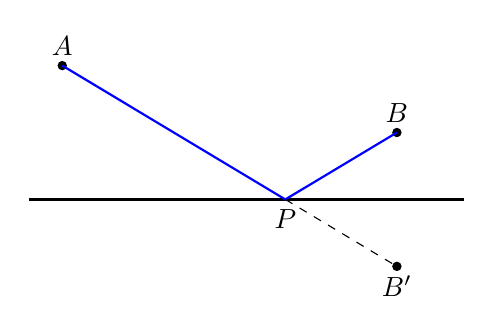
\begin{tikzpicture}[scale=.85]\draw[thick](-.5,0)--(6,0);\fill(0,2)circle(2pt)node[above]{$A$};\fill(5,1)circle(2pt)node[above]{$B$};\fill(5,-1)circle(2pt)node[below]{$B'$};\draw[blue,thick](0,2)--(3.333,0)--(5,1);\draw[dashed](3.333,0)--(5,-1);\node[below]at(3.333,0){$P$};\end{tikzpicture}
\end{center}
\section{Worked examples}
\subsection*{Example 4.1}
A=(0,2), B=(6,1) metres, reflecting line y=0. Find the shortest reflected path and reflection point.

\textbf{Solution.} $B'=(6,-1)$. Line from A to B' reaches y=0 at fraction $2/3$, so $P=(4,0)$. Length $\sqrt{6^2+3^2}=3\sqrt5$ m.
\subsection*{Example 4.2}
A rectangular sensor frame has perimeter 40 cm. Maximize its area; then impose width at most 6 cm.

\textbf{Solution.} $A=x(20-x)=100-(x-10)^2$. Unconstrained: 10 by 10 cm, 100 cm$^2$. For $0<x\le6$, closest to 10 is x=6; area $6(14)=84$ cm$^2$.
\section{Investigation}
On graph paper reflect a point across a line and measure three possible broken paths. Compare with the straight reflected construction; repeat with a restricted mirror segment.
\section{Modern application and transfer}
A periscope and folded optical instruments use mirror geometry to redirect rays within a limited enclosure. A shortest path model is useful for layout, but real designs also constrain mirror size, alignment, field of view and image quality.
\section{Source-guided reading}
SJ §7.2 (range optimization), p. 29; further reading in PHY202-A and PHY205-C.
\section{Independent practice}
\begin{enumerate}
\item \textbf{PHY101-B-4.1}. A rectangle has perimeter 28 m. Find maximum area.
\item \textbf{PHY101-B-4.2}. A=(0,3), B=(8,1), mirror y=0. Find reflection point and length.
\item \textbf{PHY101-B-4.3}. A 15 N force moves a crate 4 m. Compare work for angles 0, 60 and 90 degrees.
\item \textbf{PHY101-B-4.4}. Why might a shortest-distance route not minimize time when crossing two materials with different wave speeds? Give a counterexample using distances and speeds.
\end{enumerate}
\chapter*{References and simulations}
Tan Chien Hao (2024). \textit{Freshman Physics}.\par
Swiss Physics Olympiad Script, 3rd ed. (2019), catalogue locators pending recheck.\par
\url{https://www.math.ust.hk/~machas/differential-equations.pdf}\par
\url{https://diavn.github.io/truongchuyen/physics-curriculum.html}\par
\url{https://diavn.github.io/truongchuyen/physics-dynamics-lab.html}
\appendix
\chapter{Full solutions}
\section{Similarity and optical geometry}
\begin{enumerate}
\item \textbf{PHY101-B-1.1}. $H=18(1.5/2)=13.5$ m.
\item \textbf{PHY101-B-1.2}. $d_i=2(0.006/0.30)=0.040$ m.
\item \textbf{PHY101-B-1.3}. Normal is perpendicular to surface: $i=90^\circ-25^\circ=65^\circ=r$.
\item \textbf{PHY101-B-1.4}. Let shadow length s. Similar triangles give $3/(2+s)=1/s$, so $3s=2+s$ and $s=1$ m.
\end{enumerate}
\section{Trigonometry, vectors and navigation}
\begin{enumerate}
\item \textbf{PHY101-B-2.1}. $F_x=10$ N; $F_y=10\sqrt3$ N.
\item \textbf{PHY101-B-2.2}. Sum $(2,3)$ m; magnitude $\sqrt{13}$ m.
\item \textbf{PHY101-B-2.3}. Upstream component 3 m/s; across $\sqrt{25-9}=4$ m/s.
\item \textbf{PHY101-B-2.4}. Range 2 to 14 N. 1 N is impossible; 10 N occurs at a right angle by Pythagoras.
\end{enumerate}
\section{Graphs, gradients and accumulated quantities}
\begin{enumerate}
\item \textbf{PHY101-B-3.1}. $v=(14-2)/3=4$ m/s.
\item \textbf{PHY101-B-3.2}. $12-6=6$ m displacement; $12+6=18$ m distance.
\item \textbf{PHY101-B-3.3}. Slope $(6-2)/(0.3-0.1)=20$ V/A = 20 ohms; intercept $2-20(0.1)=0$ V.
\item \textbf{PHY101-B-3.4}. $E=100(900)=90000$ J; $100(0.25)=25$ Wh.
\end{enumerate}
\section{Geometric optimization and model transfer}
\begin{enumerate}
\item \textbf{PHY101-B-4.1}. $A=x(14-x)=49-(x-7)^2$; max 49 m$^2$ at 7 by 7.
\item \textbf{PHY101-B-4.2}. Reflect B to $(8,-1)$; fraction $3/4$ gives P=(6,0); length $\sqrt{64+16}=4\sqrt5$.
\item \textbf{PHY101-B-4.3}. $W=60\cos\theta$: 60 J, 30 J, 0 J. Net work may include other forces.
\item \textbf{PHY101-B-4.4}. Time sums $d_i/v_i$, not distances. Route A: 4 m slow region at 1 m/s and 1 m fast at 5 m/s gives 4.2 s. Route B: 1 m slow and 5 m fast gives 2 s despite 6 m versus 5 m. Actual feasible geometry must be checked.
\end{enumerate}
\end{document}
